\documentclass[11pt]{article}
\usepackage{icmlko}
\begin{document}

\title{배포가 12/12 로 넣으라 했는데 위약도 12/12 였다 --- 아래로 넓히려면 겹쳐야 한다}
\author{월드모델 실험실}
\date{노트 389 · 2026년 8월 1일}
\maketitle

\begin{abstract}
노트 388이 규칙을 하나 냈다 --- \emph{아래에서 축이 통하는 도메인은 아래를
모으면 이득이 난다.} 웹툰에서 그랬고(판 $+0.0071$ · 11/12, 위약이 이득을
통째로 지움), 만화는 노트 386이 이미 ``아래에서 축이 통한다''를 확인해 둔
도메인이다. \textbf{그래서 만화로 갔다.}

AniList \texttt{popularity\_lesser} 로 우리 바닥(633) 아래의 2025년 이전
만화 4,999편을 받아 \textbf{학습에만} 더했다(유보 258행 고정). 만화 학습이
$1{,}783 \to 5{,}647$ 이 된다.

\begin{center}
\begin{tabular}{lrrrr}
\hline
팔 & 판 차 & 부호 & 만화 차 & 부호 \\
\hline
B 아래로 넓힘 & $-0.0012$ & 4/12 & $+0.0952$ & 12/12 \\
C \textbf{위약}(새 행 라벨 섞음) & $-0.0017$ & 5/12 & $\mathbf{+0.0864}$ & \textbf{12/12} \\
\hline
\end{tabular}
\end{center}

\textbf{위약이 만화 이득의 91\%를 낸다.} 어느 행에 어느 라벨이 붙었는지를
지워도 거의 그대로다 --- 정보가 아니라 \emph{라벨 분포가 아래로 이동한
것} 자체의 효과다. 노트 387의 웹툰에서는 위약이 이득을 $+0.0305 \to
-0.0024$ 로 통째로 지웠다. \textbf{같은 처방인데 정반대다.}

\textbf{무엇이 다른가 --- 겹침이다.} 웹툰 E1의 292편은 기존 학습 범위
(최소 410) 안에 90\%가 들어가고 아래로 10\%만 넘친다. 만화의 4,999편은
\textbf{100\%가 기존 학습 최소(5,306) 아래}이고, 기존 최소와 새 최대(632)
사이에 \textbf{8.4배의 빈 구간}이 있다. 겹침이 0이다.

\textbf{그리고 규약이 이것을 못 막는다.} 판이 $-0.0012$ · 4/12 로
미결정이라 노트 378 조항 ②로 배포(팝업)를 보는데, 팝업이
$\mathbf{+0.0647}$ · \textbf{12/12} 로 \emph{넣으라} 한다. 그런데
\textbf{위약의 팝업도 $+0.0643$ · 12/12} 다. 노트 378의 구멍은 7/12
동전이었고 여기는 12/12 인데도 가짜다 --- \textbf{부호를 더 요구해서는
못 막는다.} 조항을 붙인다: \emph{학습 행을 더하는 변경은 위약이 이득을
지워야 채택한다.}
\end{abstract}

\section{쟀다}

노트 386이 만화 바닥 아래 421편(2025$+$)을 유보에 넣고 채점해 $+0.1046$
(위쪽 같은 퍼짐 창의 59번째 백분위)을 얻었다 --- \emph{아래에서 축이
통한다}. 노트 388은 웹툰에서 아래를 \emph{학습}에 넣어 판을 올렸다. 둘을
합치면 만화도 될 것 같았다.

\texttt{popularity\_lesser: 633} $+$ \texttt{startDate\_lesser: 20250101}
으로 100쪽(AniList 상한)을 받아 4,999편을 만들었다. 전부 2025년 이전이라
학습에만 들어가고 \textbf{유보 258행은 세 팔이 같다}(노트 378 조항 ④).
위약은 그 4,999편의 라벨을 자기들끼리 섞는다 --- 행 수 · 축 · 시대 분포가
전부 같고 어느 작품이 어느 라벨인지만 달라진다.

\begin{figure}[t]
\centering
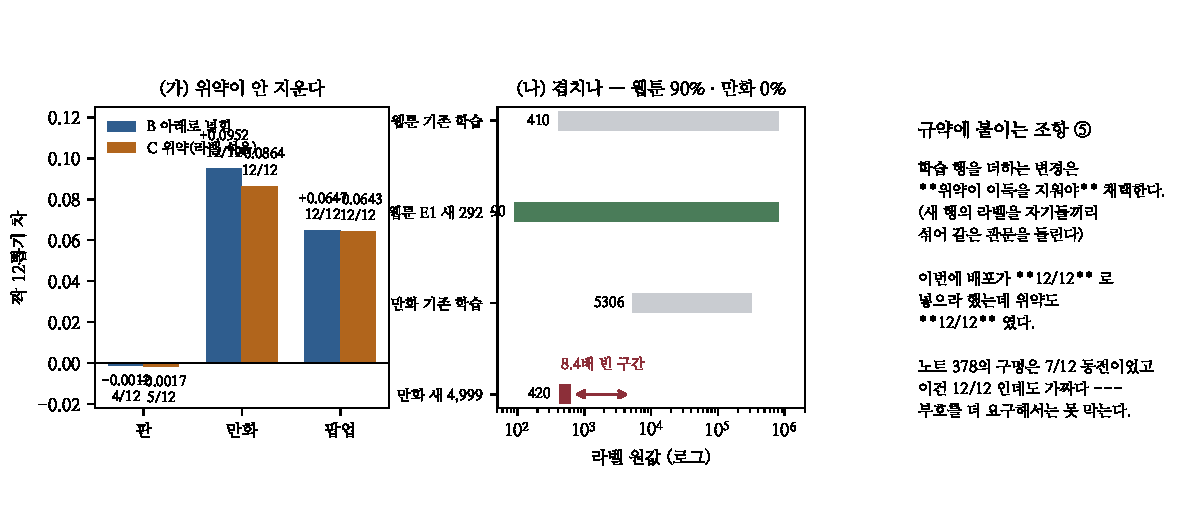
\includegraphics[width=\linewidth]{figs/fig389.pdf}
\caption{\textbf{(가)} 판 · 만화 · 팝업의 짝 12뽑기 차. 위약(주황)이
어디서나 실제 팔(파랑)을 따라온다. \textbf{(나)} 라벨 범위. 웹툰 E1은
기존 학습과 겹치고 만화의 새 행은 8.4배 떨어진 별개 구간이다.
\textbf{(다)} 규약에 붙이는 조항.}
\label{fig:main}
\end{figure}

\section{위약이 안 지운다}

만화 $+0.0952$(12/12) 대 위약 $+0.0864$(12/12). \textbf{91\%가 남는다.}

무엇이 남는지는 분명하다. 위약은 \emph{어느 행에 어느 라벨}만 지우고
\emph{어떤 라벨들이 있는지}는 그대로 둔다. 4,999편이 전부 popularity
420\,--\,632 라, 섞든 말든 학습 라벨 분포에 그 구간이 통째로 생긴다.
모형은 ``만화는 이만큼 작을 수도 있다''를 배우고 그것이 예측 눈금을 옮긴다.
\textbf{순위 상관은 눈금에 안 민감해야 하는데}, 유보 258행이 좁은 구간에
모여 있으면 눈금 이동이 순위에도 닿는다.

웹툰에서는 왜 달랐나. E1의 292편은 기존 학습 안에 90\%가 들어간다 ---
새 구간을 만드는 게 아니라 \emph{있던 구간을 촘촘하게} 한다. 그러면 라벨을
섞는 순간 이득이 사라진다(노트 387: $+0.0305 \to -0.0024$).

\begin{center}
\begin{tabular}{lrrrr}
\hline
 & 기존 학습 최소 & 새 행 범위 & 옛 최소 아래 & 위약이 지우나 \\
\hline
웹툰 E1 (노트 388) & 410 & 90\,--\,794,328 & 10\% & \textbf{지운다} \\
만화 (여기) & 5,306 & 420\,--\,632 & \textbf{100\%} & \textbf{안 지운다} \\
\hline
\end{tabular}
\end{center}

\textbf{고친 규칙: 아래로 넓히는 것이 이득이 되려면 새 라벨이 기존 범위와
겹쳐야 한다.} 완전히 떨어진 아래 덩어리는 정보가 아니라 눈금을 옮긴다.
노트 388의 문장(``아래에서 축이 통하면 아래를 모으면 이득'')에 조건이
하나 붙는다.

\section{규약이 못 막는다 --- 조항 ⑤}

판이 $-0.0012$ · 4/12 로 미결정이니 노트 378 조항 ②로 배포를 본다.

\begin{center}
팝업 $\mathbf{+0.0647}$ · \textbf{12/12} $\Longrightarrow$ 규약대로면
\textbf{채택} \\
그런데 위약의 팝업도 $\mathbf{+0.0643}$ · \textbf{12/12}
\end{center}

노트 378이 찾은 구멍은 배포가 7/12 동전으로 정하는 것이었고, 고침은
``배포도 부호 문턱을 넘어라''였다. \textbf{여기는 12/12 다.} 부호를 아무리
더 요구해도 못 막는다 --- 가짜 이득이 크고 일관되기 때문이다.

\textbf{조항 ⑤를 붙인다: 학습 행을 더하는 변경은 위약(새 행의 라벨을
자기들끼리 섞기)이 이득을 지워야 채택한다.} 노트 387이 웹툰에서 자발적으로
돌린 검사를 규약으로 올린다. 비용은 팔 하나 더 돌리는 것이고, 노트 133이
``첫 양수를 그대로 채택하지 않는다''를 열두 노트째 반복하는 것보다 싸다.

\textbf{안 채택한다.} 만화 학습 확장은 위약이 안 지우므로 넣지 않는다.
챔피언은 판 0.4423 · 분모 3,430 그대로다.

\section{남은 것}

\begin{center}
\begin{tabular}{lll}
\hline
항목 & 왜 값이 큰가 & 어떻게 \\
\hline
만화 겹치는 구간 & 633\,--\,5,306 이 비어 있다 & 그 구간만 모아 다시 관문 \\
애니 아카이브 & 무게 606 · 덮음 22\% & 수집 중 · 겹침을 먼저 본다 \\
조항 ⑤ 소급 & 지난 학습 확장에 위약이 없었다 & 노트 381 펀딩부터 \\
눈금 이동이 순위에 닿는 자리 & 유보가 좁으면 닿는다 & 유보 퍼짐과 함께 잰다 \\
\hline
\end{tabular}
\end{center}

\end{document}
